\documentclass{article}
\usepackage{amsmath}
\usepackage{tikz}
\usepackage{pgfplots}
\pgfplotsset{compat=1.16}

\begin{document}

\begin{figure}[h]
    \centering
    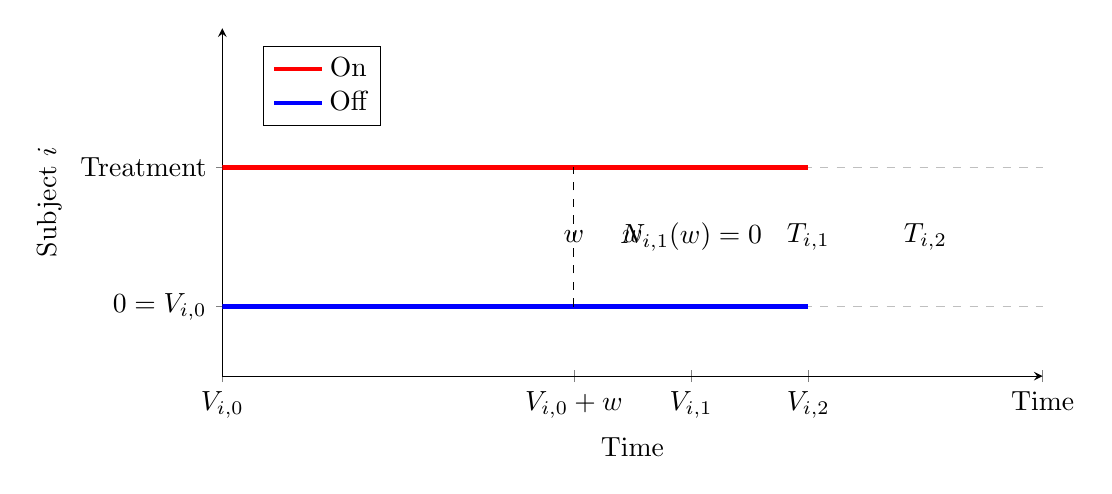
\begin{tikzpicture}
        \begin{axis}[
            axis lines=left,
            xlabel={Time},
            ylabel={Subject $i$},
            xmin=0, xmax=7,
            ymin=-0.5, ymax=2,
            xtick={0, 3, 4, 5, 7},
            xticklabels={$V_{i,0}$, $V_{i,0}+w$, $V_{i,1}$, $V_{i,2}$, Time},
            ytick={0, 1},
            yticklabels={$0 = V_{i,0}$, Treatment},
            legend pos=north west,
            ymajorgrids=true,
            grid style=dashed,
            width=12cm,
            height=6cm,
            every axis plot/.append style={ultra thick},
            every axis plot post/.append style={ultra thick},
            every axis legend/.append style={at={(0.05,0.95)}, anchor=north west},
            ]
            
            % Treatment lines
            \addplot[red] coordinates {(0,1) (5,1)};
            \addlegendentry{On};
            \addplot[blue] coordinates {(0,0) (5,0)};
            \addlegendentry{Off};
            
            % Gaping time line
            \draw[dashed, black] (3,0) -- (3,1);
            \node at (3,0.5) {$w$};
            
            % Counting process line
            \draw[blue] (3,0) -- (4,0);
            \node at (3.5,0.5) {$w$};
            \node at (4,0.5) {$N_{i,1}(w)=0$};
            
            % Time labels
            \node at (5,0.5) {$T_{i,1}$};
            \node at (6,0.5) {$T_{i,2}$};
            
        \end{axis}
    \end{tikzpicture}
    \caption{Illustration of the defined gaping time $T_{ik}$ and counting process $N_{ik}(u)$ for the subject $i$.}
    \label{fig:gaping_time_and_counting_process}
\end{figure}

\end{document}